\documentclass[../psets.tex]{subfiles}

\pagestyle{main}
\renewcommand{\leftmark}{Problem Set \thesection}
\setcounter{section}{3}

\begin{document}




\section{Determining Stereochemistry}
\marginnote{3/18:}Aflatoxin B1 is a toxin produced by a fungus which grows on a number of plant species, but is best known for causing liver carcinogenicity from contaminated peanuts.
\begin{center}
    \footnotesize
    \chemfig[fixed length=false]{*6([:60]=(-OMe)-*6(-*5(---(=O)-)=-(=O)-O-)=-*5(-*5(-=-O-)(<:[:54]H)-(<:[:-126]H)-O-)=-)}
\end{center}
The \verb|unknown-C_5.46_2025| dataset contains a series of spectra which you should be able to identify (if this is untrue, let me know and I'll send out a list). For this exercise, I'd like you to identify the ROESY crosspeaks in experiment \#9 and the NOESY crosspeaks in \#37 as follows.
\begin{enumerate}
    \item Assign all the protons in the molecule using the standard \ce{{}^13C}-directed approach.
    \begin{proof}
        {\color{white}hi}\\[1em]
        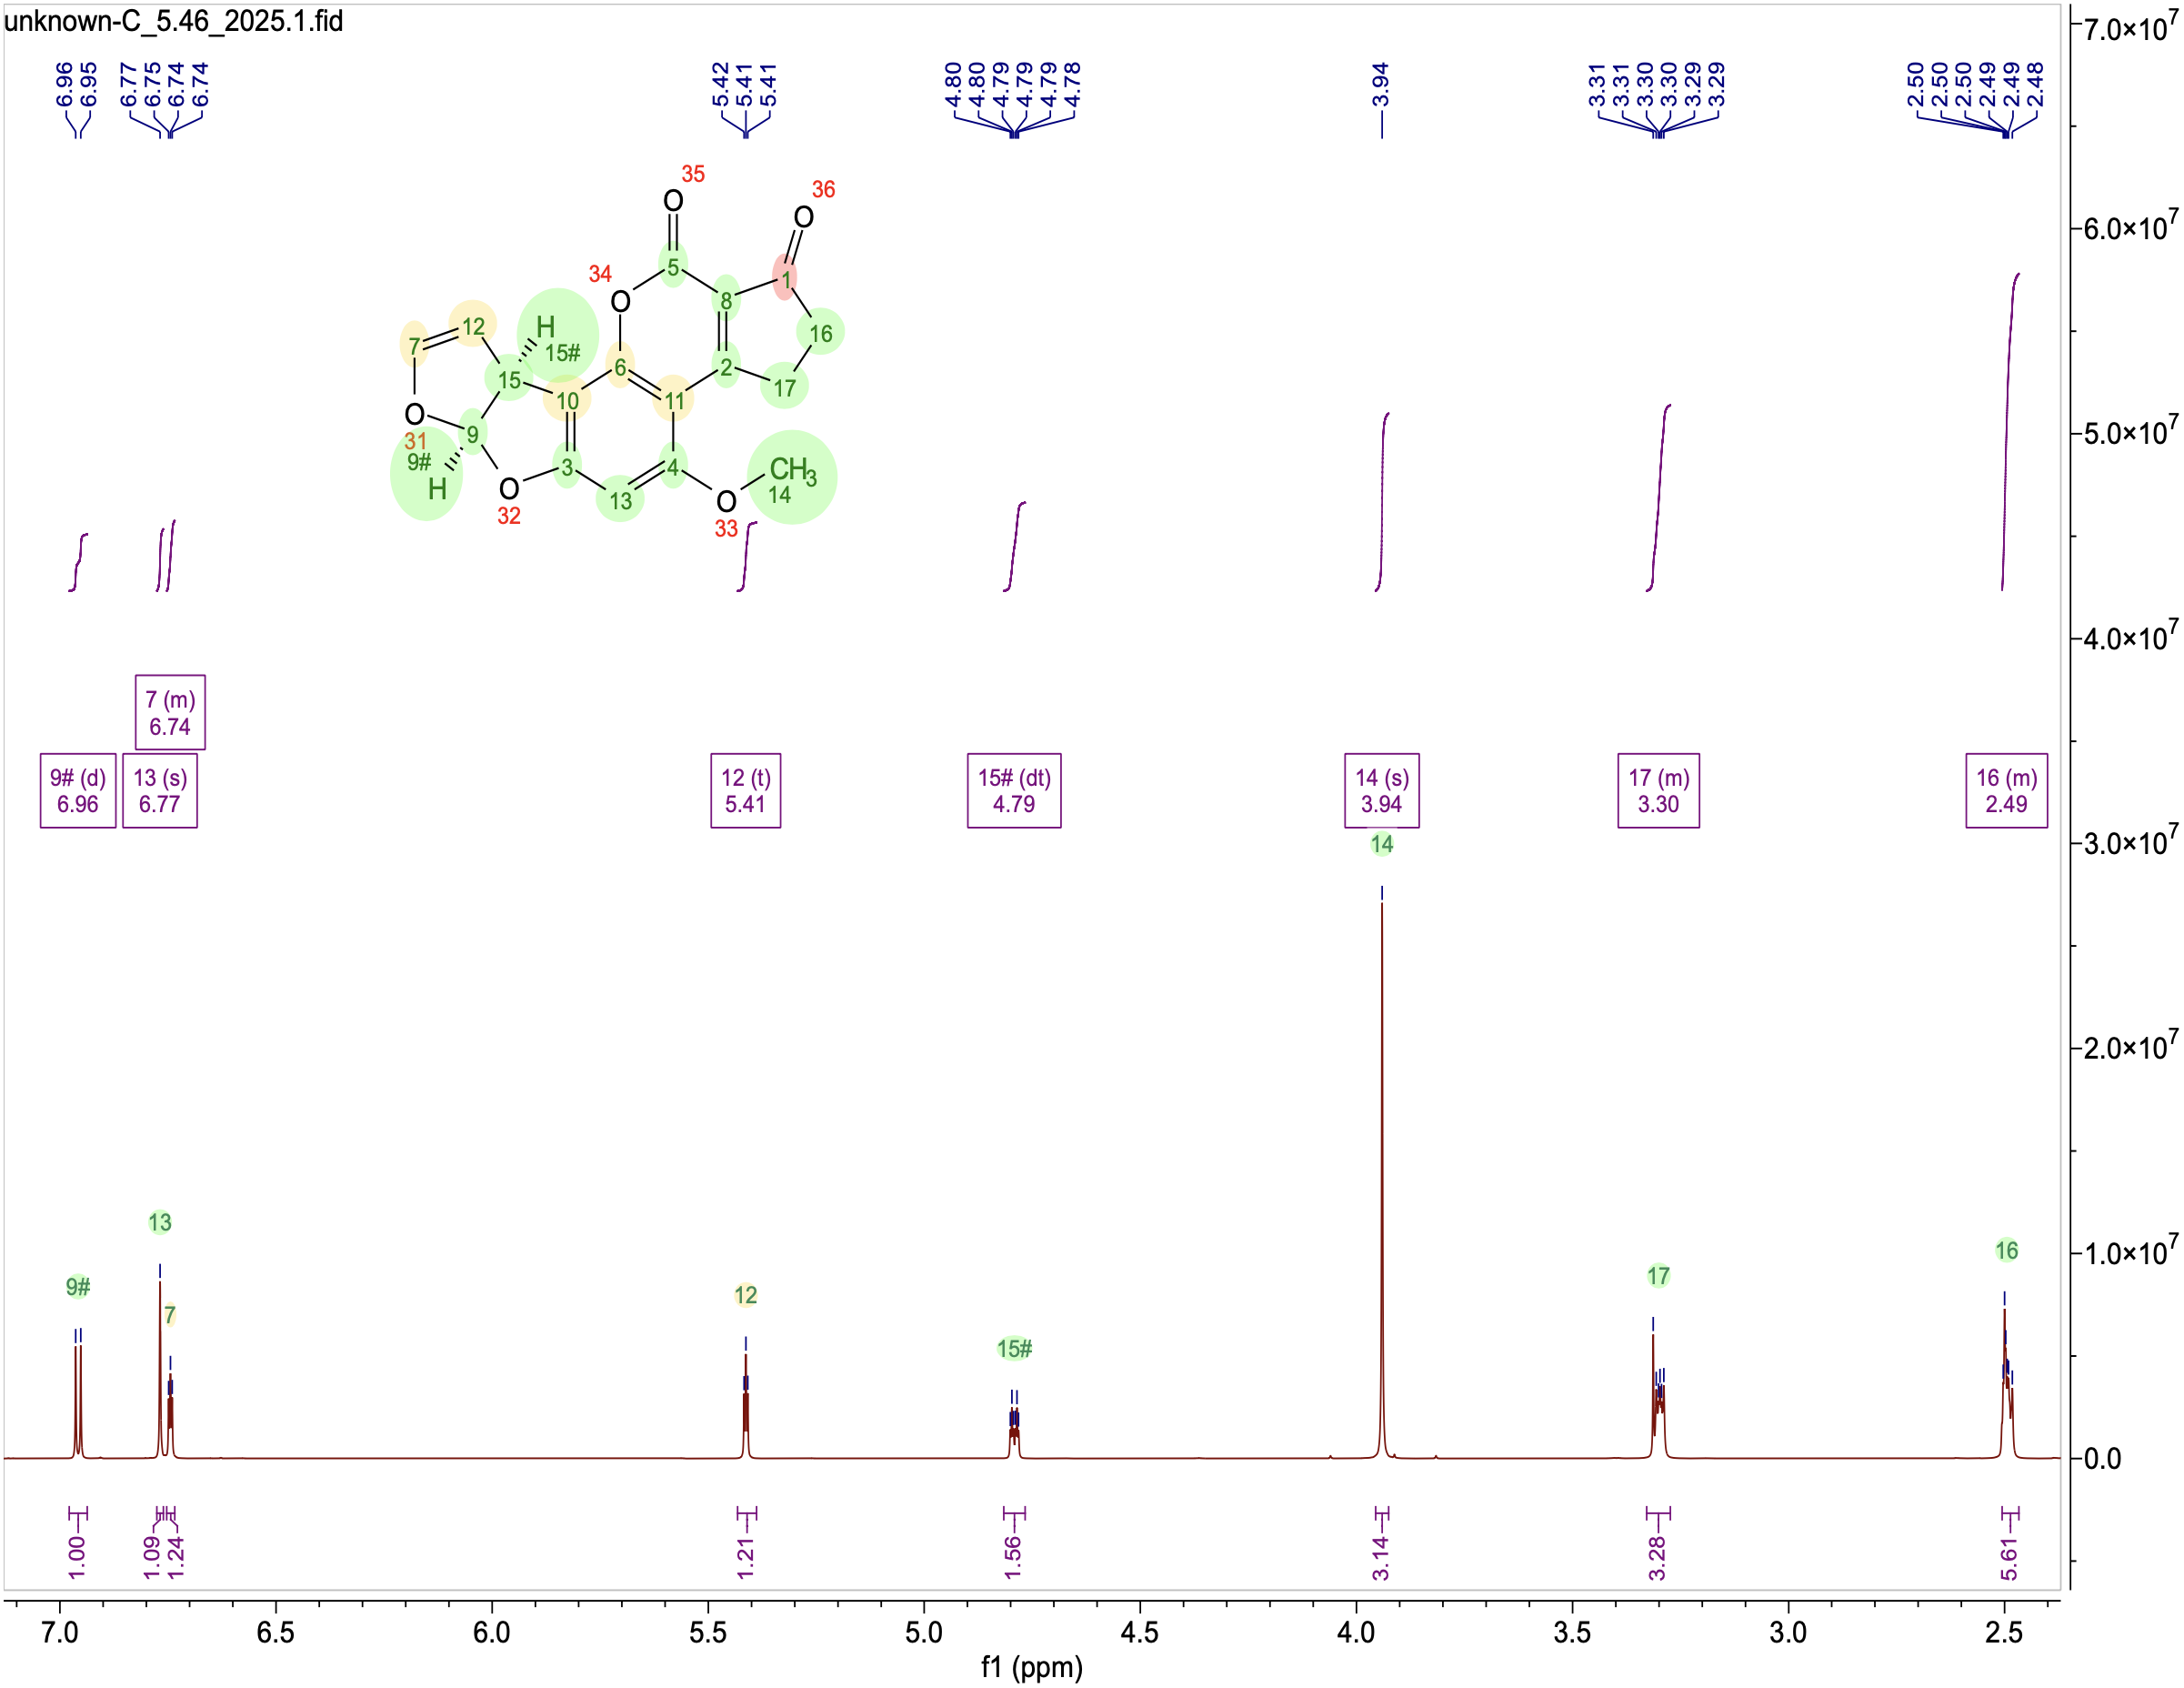
\includegraphics[width=\linewidth]{PSet4-1H.png}
        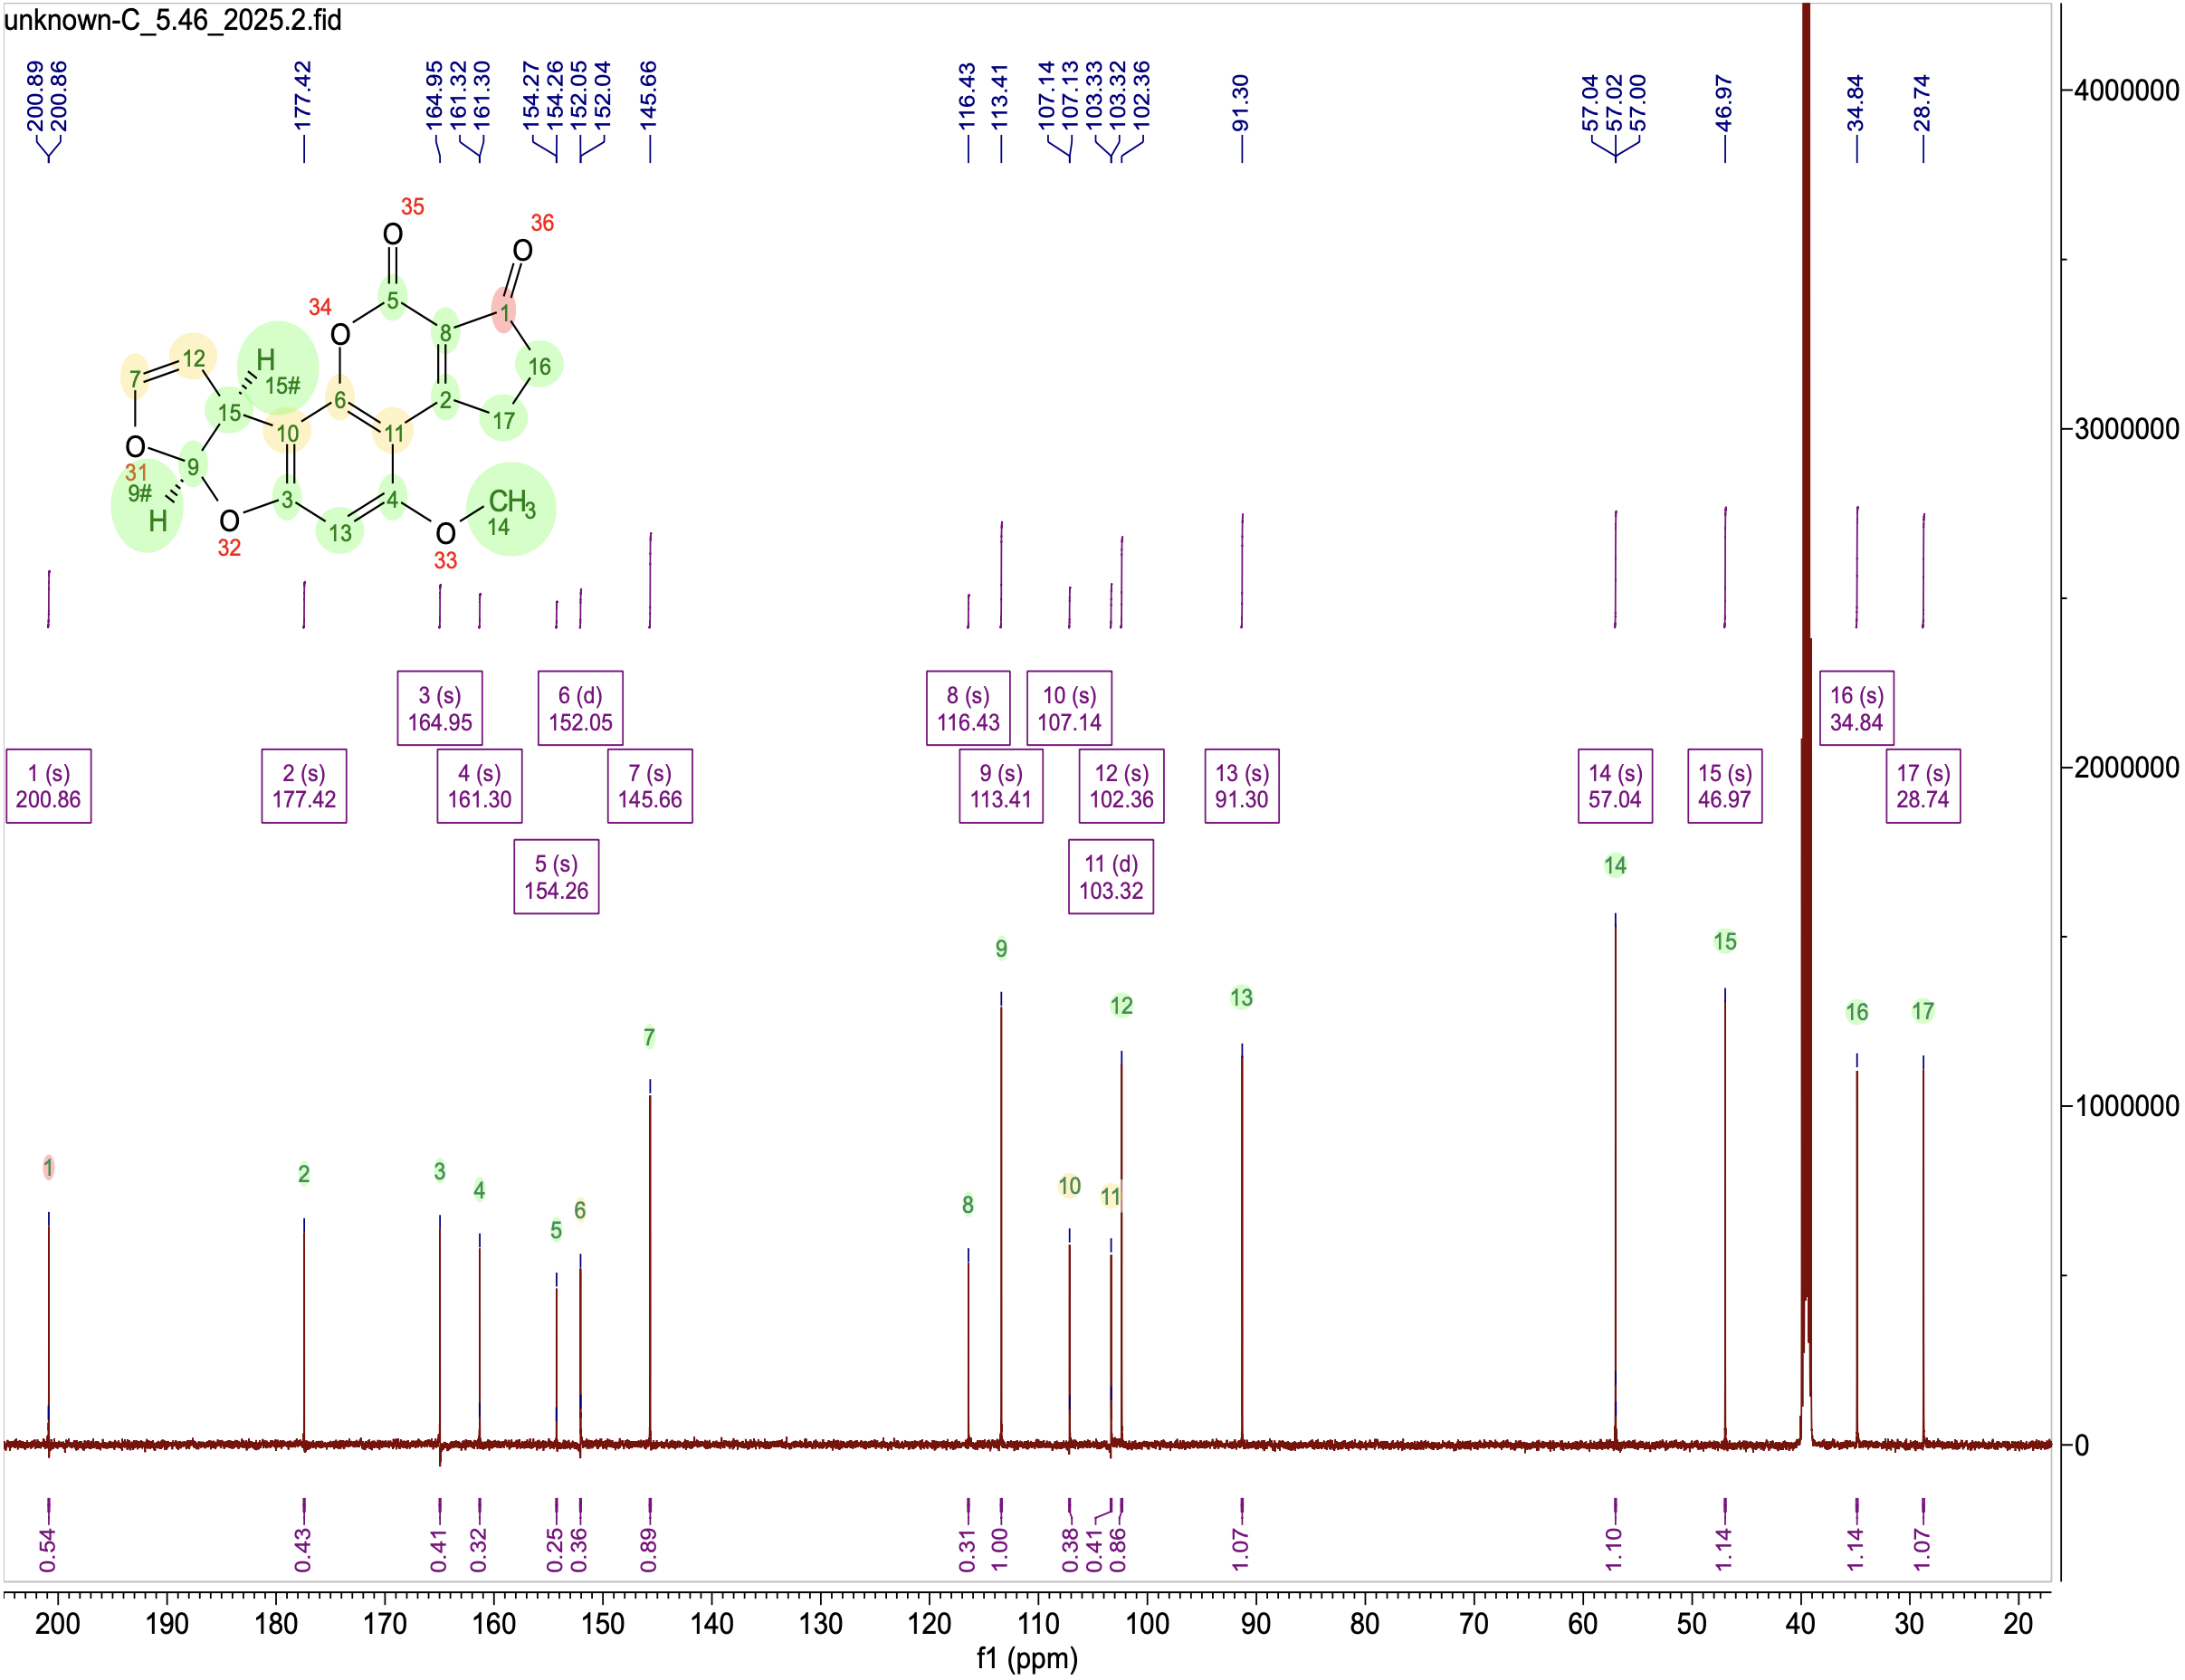
\includegraphics[width=\linewidth]{PSet4-13C.png}
    \end{proof}
    \item Show the ROE/NOE crosspeaks on the structure of Aflatoxin B1 and explain whether any are missing that you would expect.
    \begin{proof}
        {\color{white}hi}
        \begin{center}
            \footnotesize
            \chemfig[fixed length=false]{@{H13}H-[2]*6(=(-O-[:-30,,,,wvbnd](-[:30]@{H14b}H)(-[:-30]H)(-[6]@{H14a}H))-*6(-*5(-(-[:-52]@{H17b}H)(-[:-92]@{H17a}H)-(-[:20]H)(-[:-20]@{H16}H)-(=O)-)=-(=O)-O-)=-*5(-*5(-(-@{H12}H)=(-@{H7}H)-O-)(<:[:54]@{H15}H)-(<:[:-126]@{H9}H)-O-)=-)}
            \chemmove{
                \draw [noesy=2pt] (H7) to[bend left=20] node[above,xshift=-2pt]{7-12} (H12);
                \draw [noesy=2pt] (H12) to[bend left=20] node[right,yshift=2pt]{12-15} (H15);
                \draw [noesy=2pt] (H15) to[bend right=20] node[left,xshift=3pt,yshift=4pt]{15-9} (H9);
                \draw [noesy=2pt] (H13) to[bend right=20] node[below]{13-14} (H14a);
                \draw [noesy=2pt] (H14b) to[bend right=30] node[right]{14-17} (H17a);
                \draw [noesy=2pt] (H17b) to[bend right=20] node[right,yshift=-3pt,xshift=-2pt]{17-16} (H16);
            }
        \end{center}
        Some cross peaks are small, but all the ones I expect to see are distinguishable from noise at some level of zoom on both spectra. The 14-17 crosspeak is the hardest to distinguish on both spectra.
    \end{proof}
    \item Confirm the stereochemistry of the bridged ring.
    \begin{proof}
        Since we can observe a significant 15-9 NOESY, the saturated bridgehead carbons on the western fragment of Aflatoxin B1 must bear two \emph{cis} protons. Without a chiral resolving reagent, it is impossible to determine the absolute stereochemistry of the molecule.
    \end{proof}
    \item Experiment \#13 shows a \ce{{}^1H}-\ce{{}^13C} HSQC in which the decoupling is turned off during acquisition; indicate on the structure which proton-carbon couplings are larger than usual and explain why you think this is.
    \begin{proof}
        To begin, here is an accounting of all ${}^1J_\text{CH}$ coupling constants in the visible in the coupled HSQC spectrum.
        \begin{table}[H]
            \centering
            \small
            \renewcommand{\arraystretch}{1.2}
            \begin{tabular}{|c|c|c|}
                \toprule
                \textbf{Proton \#} & \textbf{Shift (ppm)} & $\bm{{}^1J_\textbf{CH}}$ \textbf{(Hz)}\\
                \midrule
                9  & 6.96 & 188.41\\
                13 & 6.77 & 167.62\\
                7  & 6.74 & 202.33\\
                12 & 5.41 & 181.30\\
                15 & 4.79 & 146.88\\
                14 & 3.94 & 146.80\\
                17 & 3.30 & 139.69\\
                16 & 2.49 & 132.41\\
                \bottomrule
            \end{tabular}
        \end{table}
        The largest proton-carbon coupling constant corresponds to an $sp^2$-hybridized carbon-proton bond, as we might expect since increasing $s$-character means shorter bonds and more coupling. However, with all of the strain in this molecule, it is very difficult to qualitatively predict the magnitude of the ${}^1J_\text{CH}$ couplings.
    \end{proof}
\end{enumerate}




\end{document}